\section{Nominal MPC}
 
\subsection{CITOC: what we would like to solve}

\begin{gather*}
    J^*_\infty(x(0)) = \underset{u(\cdot)}{\mathrm{min}}\sum^\infty_{i=0}I(x_i,u_i) \\
    \mathrm{subj.\hspace{2mm} to} \hspace{3mm}x_{i+1} = Ax_i + B u_i, i = 0,\dots,\infty \\
    x_i \in \mathcal{X}, u_i \in \mathcal{U}, i = 0,\dots,\infty\\
    x_0 = x(0)
\end{gather*}

\begin{itemize}
    \item \textbf{state cost} $I(x,u)$: cost of being in state x and applying input u.
\end{itemize}
\subsection{CFTOC: what we can sometimes solve}
\begin{gather*}
    J^*_{k\rightarrow k+N|k}(x(k)) = \underset{U_k\rightarrow k+ N|k}{\mathrm{min}} \textcolor{red}{I_f(x_{k+N|k})}+ \sum^{\textcolor{red}{N-1}}_{i=0}I(x_{k+i|k, u_{k+i|i}}) \\ 
    \mathrm{subj. \hspace{2mm} to \hspace{2mm}} x_{k+i+1|k}= Ax_{k+i|k} + Bu_{k+i|k} i = 0,\dots,N-1 \\
    x_{k+i|k} \in \mathcal{X}, u_{k+i|k} \in \mathcal{U}, i= 0,\dots,N-1 \\
    \textcolor{red}{x_{k+N|k} \in \mathcal{X}_f}\\
    x_{k|k} = x(k)
\end{gather*}
where $U_{k\rightarrow k + N|k}= \{u_{k|k}\dots,u_{k+N-1|k}\}$
\begin{itemize}
    \item $I_f(x_{k+N|k})$: approximates the 'tail' of the cost
    \item $\mathcal{X}_f$: Approximates the tail of the constraints 
\end{itemize}
\subsection{MPC: Mathematical Formulation}
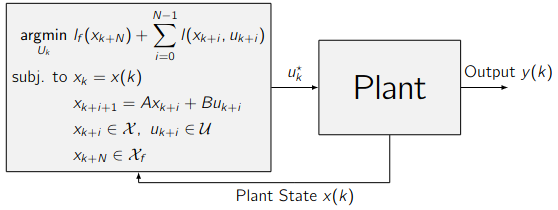
\includegraphics[width = \linewidth]{MPC_summary/Images/Screenshot from 2021-07-30 16-13-03.png}
\subsection{constrained Linear Optimal Control}
Cost function \[J(x_0,U) = I_f(x_N)+\sum^{N-1}_{i=0} I (x_i,u_i)\]
\begin{itemize}
    \item Squared  Euclidian norm: $I_f(x_N)=x_N^TPx_N$ and $I(x_i,u_i ) = x_i^TQx_i+u^T_iRu_i, \mathrm{with} P \succeq 0, Q\succeq 0, R\succ 0$
\end{itemize}
\subsection{Transform Quadratic Cost CFTOC $\Rightarrow$ QP}
\begin{gather*}
    J^*(x(k)) = \underset{U}{\mathrm{min}}x^T_NPx_N+ \sum^{N-1}_{i=0}x_i^TQx_i + u_j^TRu_i \\ 
    \mathrm{subj. \hspace{2mm} to \hspace{2mm}} x_{i+1}= Ax_{i} + Bu_{i} i = 0,\dots,N-1 \\
    x_{i} \in \mathcal{X}, u_i \in \mathcal{U}, i= 0,\dots,N-1 \\
    {x_{N} \in \mathcal{X}_f}\\
    x_{0} = x(k)\\
    \Downarrow\\
    \underset{z\in\mathbb{R}^n}{\mathrm{min}}\frac{1}{2}z^THz +q^Tz +r\\
    \mathrm{subj. \hspace{2mm} to\hspace{2mm} Gz\leq h}\\
    Az = b
\end{gather*}
\subsubsection{by substitution}
\begin{gather*}
    J^*(x(k)) = \underset{U}{\mathrm{min}} [U^Tx(k)^T]
    \tiny{\begin{bmatrix}
    H & F^T\\
    F & Y
    \end{bmatrix}} [U^Tx (k)^T ]^T\\ 
    \mathrm{subj.\hspace{2mm} to\hspace{2mm}} GU \leq w + E x(k)
\end{gather*}
